\graphicspath{{chapters/06/images/}}
\chapter{Hybrid simulation approaches}

\section{Introduction}
Hybrid simulation approaches refer to a class of methods that combines the advantages of complementary simulation approaches: the system is partitioned into subsystems that are simulated with different methods.
When exact stochastic simulation is not a realistic option approximate strategies have to be considered together with their accuracy, so they often require the fulfilment of specific conditions.
The state space associated with biochemical reaction networks can be partitioned into regions depending on the nature of the system, according to the number of molecules and the frequency of reaction events.
This helps evaluate which approximations are reasonable.
The essential elements are the abundance of the species and the frequency of reaction.
Threshold variables demarcate the different partitions and they are model dependents as seen in figure \ref{fig:regions}:

\begin{multicols}{2}
  \begin{itemize}
    \item $t_1$ indicates whether a reaction is considered fast.
    \item $t_2$ indicates whether a population is abundant or not.
    \item $t_3$ and $t_4$ the border between stochastic variation and deterministic behaviour.
  \end{itemize}
\end{multicols}

\begin{figure}[H]
  \centering
  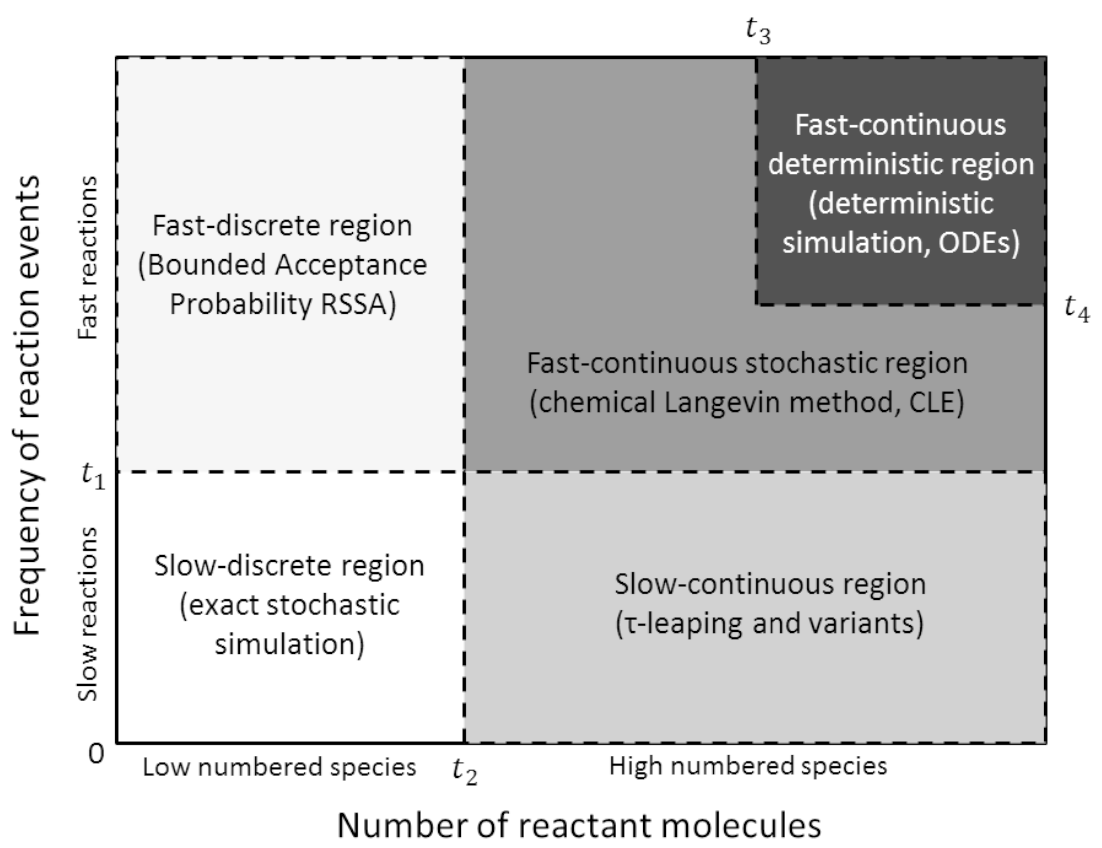
\includegraphics[width=0.5\textwidth]{regions.png}
  \caption{Partitions of the state space}
  \label{fig:regions}
\end{figure}

  \subsection{Slow-discrete region}
  The system is in a slow-discrete region when the reaction are slow and low numbered species are present.
  The species must be represented with an integer and discrete changes are allowed.
  Moreover the reaction events are rare and correspond to significant changes in the system.
  This region should be treated with the highest accuracy method available.

  \subsection{Fast-discrete region}
  The system is in the fast-discrete region whenever molecular populations are small and the reactions happen frequently enough that exact simulation could be intractable.
  This region can be treated with stochastic approximate algorithms developed to work with large reaction propensities and small populations like BA-RSSA.

  \subsection{Slow-continuous region}
  The system is in the slow-continuous region whenever molecular population are large and reaction are slow.
  The molecular populations can be assumed continuous and each reaction occurrence does not change significantly its species concentration.
  The simulation of many reaction occurrences can be skipped without affecting the accuracy.
  This region can be treated by the $\tau$-leaping algorithm.

  \subsection{Fast continuous stochastic and deterministic region}
  The system starts in the fast continuous stochastic and goes into the deterministic whenever it has fast reactions and high number species.
  In the first case the CLE can be considered for the simulation, while in the second deterministic simulations can be used.

  \subsection{Dimensionality explosion}
  The system is two dimensional only when it has one species and one reaction.
  When these two sets increase the criteria above can be applied only when all of them belong to the same region.
  This is a very strict condition that must be preserved along all of the simulation process.
  Hybrid simulation approaches try to solve this problem by dividing the system into parts that fit with the regions described which are then simulated by ad hoc simulation methods to provide the best compromise between accuracy and runtime.

\section{Reaction-based system partitioning}
The reaction based system partitioning partitions the system into subnetwork that reaquire to be simulated by the same strategy.
The reaction are divided into $\mathcal{R}^s$ and $\mathcal{R}^f$ of slow and fast reactions.
Fast reaction have high propensities and can be simulated by CLE or deterministic simulation while slow one have low propensities.
When deterministic simulation is employed a preliminary step is required to transform the set of reactions in ODEs.
Slow reactions require a more accurate stochastic simulation approache.

  \subsection{Classifying fast reactions}
  Reactions can be fast when it occurs many times in a small time interval and the effect of each reaction on the number of reactants and products is small, so quantitatively:

  $$a_j\tau^f \ge \theta\ll 1$$

  And:

  $$\vec{x}_i > \lambda|\vec{v}_{ij}|, \forall S_i\in Reactants(R_j)\cup Products(R_j)$$

  $\theta$ and $\lambda$ define the minimum number of time a fast reaction can be applied within $\tau^f$ and how fine grained the species must be in order for them to appear as continuous.
Usually for practical models $\theta = 10$ and $\lambda = 100$.

  \subsection{Partitioning algorithm}
  An implementation of this reaction-based partitioning can be found in algorithm \ref{algo:two-class-reaction-partitioning}

  \begin{algorithm}[H]
\DontPrintSemicolon
\SetKwComment{comment}{$\%$}{}
\SetKw{Int}{int}
\SetKw{To}{to}
\SetKw{Return}{return}
\SetKw{Not}{not}
\SetKw{Input}{Input}
\SetKw{Output}{Output}
\SetKw{False}{false}
\SetKw{True}{true}
\SetKwData{Item}{item}
\SetKwFunction{Min}{min}
\SetKwFunction{TitleFunction}{Two class reaction-based partitioning}

\caption{\protect\TitleFunction{}}
\label{algo:two-class-reaction-partitioning}

\Input: a biochemical reaction system with stoichiometrix matrix $\vec{v}$ and current state $\vec{x}$, the time increment $\tau^f$ for the approximate simulation of fast reaction, $\theta$ defining the minimum number of times that a fast reaction has to be applied on average within $\tau^f$ and $\lambda$ indicating how fine grained the reactant and product species must be in order to be approximated by continuous numbers\;

\Output: the sets $\mathcal{R}^s$ and $\mathcal{R}^f$\;

$\mathcal{R}^s = \emptyset$\;
$\mathcal{R}^f = \emptyset$\;

\ForEach{$R_j\in\mathcal{R}$}{
	\If{$a_j\tau^f<\tau$}{
		$R_j\in\mathcal{R}^s$\;
	}
	\ElseIf{$\exists S_i\in Reactants(R_j)\cup Products(R_j): \vec{x}_i\le\lambda|\vec{v}_{ij}|$}{
		$R_j\in\mathcal{R}^s$\;
	}
	\Else{
		$R_j\in\mathcal{R}^f$\;
	}
}
\end{algorithm}


  \subsection{Dynamic partitioning}
  Because reaction propensities and state vector change in time the partitioning has to be evaluated during the simulation.
  This is dynamic partitioning.
  It is important when the system state varies considerably over time.
  A fixed partitioning can be used  when the subsystems are different and these differences remain constant during the simulation.

  \subsection{Different constraints}
  Some partitioning strategies depends only on the second condition and relax it to include only the reactants.
  This is to speed up the simulation by taking out the stochastically simulated fast reaction subsystem, while particle-number based partitioning is concerned with correctly treating reactions with small concentrations.
  Moreover $\tau^f$ can change at each simulation step and can be not considered: the reaction are divided into a tentative partitioning and then a fixed point iterative scheme happens, tuning the partitioning so that the propensity of each fast reaction will be at least $\lambda$ times larger than the fastest slow reaction.
  This procedure, outlined in algorithm \ref{algo:two-class-reaction-fixed-point} is more computationally demanding but has less parameters.

  \begin{algorithm}[H]
\DontPrintSemicolon
\SetKwComment{comment}{$\%$}{}
\SetKw{Int}{int}
\SetKw{To}{to}
\SetKw{Return}{return}
\SetKw{Not}{not}
\SetKw{Input}{Input}
\SetKw{Output}{Output}
\SetKw{False}{false}
\SetKw{True}{true}
\SetKwData{Item}{item}
\SetKwFunction{Min}{min}
\SetKwFunction{TitleFunction}{Two class reaction-based partitioning with fixed point iterations}

\caption{\protect\TitleFunction{}}
\label{algo:two-class-reaction-fixed-point}

\Input: a biochemical reaction system with stoichiometrix matrix $\vec{v}$ and current state $\vec{x}$, the time increment $\tau^f$ for the approximate simulation of fast reaction, $\gamma$ indicating how fine grained the reactant and product species must be in order to be approximated by continuous numbers abd $\lambda$ indicating how many times the propensity of the slowest fast reaction has to be larger than the propensity of the fastest slow reaction\;

\Output: the sets $\mathcal{R}^s$ and $\mathcal{R}^f$\;

$a^s_{\max} = 0$\;
$\mathcal{R}^s = \emptyset$\;
$\mathcal{R}^f = \emptyset$\;

\ForEach{$R_j\in\mathcal{R}$}{
	\If{$\exists S_i\in Reactants(R_j)\cup Products(R_j): \vec{x}_i\le\gamma|\vec{v}_{ij}|$}{
		$R_j\in\mathcal{R}^s$\;
		$a_{\max}^s = \max\{a_{\max}^s, a_j\}$\;
	}
	\Else{
		$R_j\in\mathcal{R}^f$\;
	}
}

\If{$\mathcal{R}^s\neq\emptyset\land\mathcal{R}^f\neq\emptyset$}{
	\Repeat{$fxdpt = $\True}{
		fxdpt = \True\;
		\ForEach{$R_j\in\mathcal{R}^f$}{
			\If{$a_j<\lambda a_{\max}^s$}{
				move $R_j$ from $\mathcal{R}^f$ to $\mathcal{R}^s$\;
				$a_{\max}^s = \max\{a_{\max}^s, a_j\}$\;
				fxdpt = \False\;
			}
		}
	}
}
\end{algorithm}


  \subsection{Four class reaction partitioning}
  The reaction partitioning in two classes reduces at minimum the simulation strategies implemented in the hybrid algorithm, simplifying its implementation, but reducing the accuracy of the results.
  A higher number of reaction classes are introduced to be more consistent with the regions.
  A way of doing so is to divide it into fours set:

  \begin{multicols}{2}
    \begin{itemize}
      \item Very slow reactions $\mathcal{R}^{vs}$ requiring exact simulation.
      \item Slow reactions $\mathcal{R}^s$ requiring a $\tau$-leaping method.
      \item Medium reactions $\mathcal{R}^m$, requiring CLE.
      \item Fast reactions $\mathcal{R}^f$, requiring deterministic simulation.
    \end{itemize}
  \end{multicols}

  At the basis of this strategy is the computation of $\tau$, providing the next firing time of a model reaction and imposing the following restraints:

  \begin{itemize}
    \item $a_j\tau\le 1$ $R_j$ very slow.
    \item $a_j\tau > 1\land a_j\tau\not\gg 1$ $R_j$ is slow.
    \item $a_j\tau\gg 1\land\sqrt{a_j\tau}\not\gg 1$ $R_j$ is medium.
    \item $\sqrt{a_j\tau}\gg 1$ $R_j$ is fast.
  \end{itemize}

    \subsubsection{Algorithm}
    An implementation of the four class reaction based partitioning is outlined in algorithm \ref{algo:four-class-reaction}, introducing $\theta$ to implement the $\gg$ constraint

    
\begin{algorithm}[H]
\DontPrintSemicolon
\SetKwComment{comment}{$\%$}{}
\SetKw{Int}{int}
\SetKw{To}{to}
\SetKw{Return}{return}
\SetKw{Not}{not}
\SetKw{Input}{Input}
\SetKw{Output}{Output}
\SetKw{False}{false}
\SetKw{True}{true}
\SetKwData{Item}{item}
\SetKwFunction{Min}{min}
\SetKwFunction{TitleFunction}{Four class reaction-based partitioning}

\caption{\protect\TitleFunction{}}
\label{algo:four-class-reaction-partitioning}

\Input: a biochemical reaction system with current staet $\vec{x}$, the firing time $\tau$ of the next model reaction and the threshold parameter $\theta$\;

\Output: the sets $\mathcal{R}^{vs}$, $\mathcal{R}^s$, $\mathcal{R}^m$ and $\mathcal{R}^f$\;

$\mathcal{R}^{vs} = \emptyset$\;
$\mathcal{R}^f = \emptyset$\;
$\mathcal{R}^m = \emptyset$\;
$\mathcal{R}^f = \emptyset$\;

\ForEach{$R_j\in\mathcal{R}$}{
	\If{$a_j\tau\le 1$}{
		$R_j\in\mathcal{R}^{vs}$\;
	}
	\ElseIf{$a_j\tau < \theta$}{
		$R_j\in\mathcal{R}^s$\;
	}
	\ElseIf{$\sqrt{a_j\tau} < \theta$}{
		$R_j\in\mathcal{R}^m$\;
	}
	\Else{
		$R_j\in\mathcal{R}^f$\;
	}
}
\end{algorithm}


\section{Synchronization of exact and approximate simulations}
When the hybrid strategy moves forward one simulation step, slow reaction are simulated by exact stochastic simulation while less accurate strategies are used for faster reactions.
The approximate simulation of faster reactions is constrained to not exceed the firing time of the first slow reaction.
This is a synchronization to preserve the accuracy of the simulation.
Even if the simulation of slow reactions is exact, their firing is not guaranteed to be exact when faster reactions are simulated in an approximate way.
Since the approximation is difficult to obtain many hybrid algorithm implement a simulation for slow reactions that is not exact, but less approximate than the one of the fast reactions.

  \subsection{Algorithm}
  An implementation of a four class hybrid simulation strategy is implemented in algorithm \ref{algo:four-class-hybrid-simulation}.

  \begin{algorithm}[H]
\DontPrintSemicolon
\SetKwComment{comment}{$\%$}{}
\SetKw{Int}{int}
\SetKw{To}{to}
\SetKw{Return}{return}
\SetKw{Not}{not}
\SetKw{Input}{Input}
\SetKw{Output}{Output}
\SetKw{False}{false}
\SetKw{True}{true}
\SetKwData{Item}{item}
\SetKwFunction{Min}{min}
\SetKwFunction{Partitioning}{partitioning}
\SetKwFunction{TitleFunction}{Four class hybrid simulation strategy}

\caption{\protect\TitleFunction{}}
\label{algo:four-class-hybrid-simulation}

\Input: a biochemical reaction system with initial state $X_0$, the simulation ending time $T_{\max}$ and the threshold parameter $\theta>1$\;

\Output: a trajectory of the biochemical system\;

$t = 0$\;
$X = X_0$\;

\While{$t<T_{\max}$}{
	compute $\tau$ according to the $\tau$-leaping method\;
	\Repeat{$\neg updateNeeded$}{
		$updateNeeded$ = \False\;
		\ForEach{$R_j\in\mathcal{R}$}{
			$\mathcal{R}^{vs}, \mathcal{R}^s, \mathcal{R}^m, \mathcal{R}^f$ = \Partitioning{$\mathcal{R}$, $\theta$, $\tau$}\;
		}
		\ForEach{$R_j\in\mathcal{R}^{vs}$}{
			compute $\tau_f$ using exact simulation algorithm\;
		}
		\If{$\mathcal{R}^{vs} = \mathcal{R}\land \tau\neq\min\{\tau_j\}, R_j\in\mathcal{R}^{vs}$}{
			$\tau = \min\{\tau_j\}, R_j\in\mathcal{R}^{vs}$\;
		}
		\If{$\tau>\min\{\tau_j\}, R_j\in\mathcal{R}^{vs}$}{
			$\tau = \min\{\tau_j\}, R_j\in\mathcal{R}^{vs}$\;
			$updateNeeded$ = \True\;
		}
		\If{$\neg updateNeeded$}{
			compute $X^{new}$ at $t+\tau$ approximating the firing of reactions in $\mathcal{R}^s. \mathcal{R}^m, \mathcal{R}^f$ accorrding to:\;
			$\tau$-leaping method for slow reactions\;
			CLE for medium reactions\;
			deterministic simulation for fast reactions\;
			update $X^{new}$ by applying $R_j\in\mathcal{R}^{vs}$, such that $\tau_j = \tau$\;
			\If{any $X_i^{new}<0$}{
				$\tau = \frac{\tau}{2}$\;
				$updateNeeded$ = \True\;
			}
			\Else{
				$X = X^{new}$\;
				$t = t+\tau$\;
			}
		}
	}
}
\end{algorithm}


  \subsection{Preserving the exactness}
  In order to preserve the exactness of the simulation of slow reactions, the reaction probability density has to be extended to consider time-varying transition propensities account for the propensities of slow reactions that change due to the simulation of fast reactions.
  The pdf of the next firing of a slow reaction $R_\mu\in\mathcal{R}^s$ becomes:

  $$p^s(\tau, \mu|\vec{x}, t) = a_\mu(X(t+\tau))e^{-\int_t^{t+\tau}a_0^s(X(t'))dt'}$$

  Where $X(t+\tau)$ is the system at time $t+\tau$, $\vec{x}$ is the current system state and:

  $$a_0^s = \sum\limits_{R_j\in\mathcal{R}^s}a_j$$

  The firing time of the next slow reaction is obtained by solving:

  $$\int_t^{t+\tau} a_0^s(X(t'))dt' = -\ln(r)$$

  This solution is difficult to compute: the system state is changed by fast reactions during the time interval.
  The hybrid simulation has to evaluate it simultaneously with the simulation of the fast reaction to generate the next slow reaction event.

    \subsubsection{Event detection}
    In order to satisfy the time integral the simulation of fast reaction has to include an event detection part.
    The easiest way to do so is to relax the constraint of the equation to find a time instant along the simulation such that:

    $$\biggr\vert\int_t^{t+\tau}a_0^x(X(t'))dt' + \ln(r)\biggr\vert\le\epsilon$$

    Where $\epsilon\approx 0$ is a positive error threshold.
    This makes the simulation of slow reaction depend on $\epsilon$.
    This correspond to adding to the set of deterministic ODEs an additional equation:

    $$\frac{dRES}{dt} = a_0^xRES(0) = \ln(r)$$

    This is numerically integrated together with the set of ODE until $|RES(t+\tau)|\le\epsilon$.
    The computation of the firing time of the next slow reaction will be not exact because it depends on the order of the numerical method used to solve the initial value problem.

    \subsubsection{Algorithm}
    A two class hybrid strategy with exact simulation of slow reactions is outlined in algorithm \ref{algo:two-class-hybrid-exact-slow}

    \begin{algorithm}[H]
\DontPrintSemicolon
\SetKwComment{comment}{$\%$}{}
\SetKw{Int}{int}
\SetKw{To}{to}
\SetKw{Return}{return}
\SetKw{Not}{not}
\SetKw{Input}{Input}
\SetKw{Output}{Output}
\SetKw{False}{false}
\SetKw{True}{true}
\SetKwData{Item}{item}
\SetKwFunction{Min}{min}
\SetKwFunction{Partitioning}{partitioning}
\SetKwFunction{TitleFunction}{Two class hybrid strategy with exact simulation of slow reactions}

\caption{\protect\TitleFunction{}}
\label{algo:two-class-hybrid-exact-slow}

\Input: a biochemical reaction system with initial state $X_0$, the simulation ending time $T_{\max}$\;

\Output: a trajectory of the biochemical system\;

$t = 0$\;
$X = X_0$\;

\While{$t<T_{\max}$}{
	\ForEach{$R_j\in \mathcal{R}$}{
		$\mathcal{R}^s, \mathcal{R}^f$ = \Partitioning{$\mathcal{R}$}\;
	}
	generate two uniform random numbers $r_1, r_2\sim norm(0,1)$\;
	compute $X_{new}$ from $X$ by approximating the firing of fast reactions until $t+\tau$ is reached that satisfied the integral $\int_t^{t+\tau} a_0^s(X(t'))dt' +\ln(r) = 0$\;
	select the slow reaction $R_\mu\in\mathcal{R}^s$ with the smallest $\mu$ such that $\sum\limits_{j=1}^\mu a_j>r_2a_0^s$\;
	update $X_{new}$ by applyinh $R_\mu$\;
	$t = t+\tau$\;
}
\end{algorithm}


\section{Hybrid Rejection-Based SSA}
The hybrid rejection based stochastic simulation algorithm HRSSA is built on top of RSSA.
The simulation strategy relies on the concept of fluctuation interval:

$$[\underline{\vec{x}}, \overline{\vec{x}}] = [(1-\delta)\vec{x}, (1+\delta)\vec{x}], 0<\delta<1$$

Used to obtain exact stochastic simulation of slow reactions without computing the integral, improving simulation accuracy and runtime.

  \subsection{Reaction partitioning}
  Reactions are partitioned in two classes and the partition is updated only when the current system does not fit any more in its fluctuation interval: the partitioning is done considering the lower bond $\underline{\vec{x}}$.
  This does not affect the accuracy of the classification, but it imposes more stringent constraints that increase the number of reactions classified as slow.

  \subsection{Firing time}
  The sum of the upper propensity bounds of slow reactions is computed:

  $$\overline{a_0}^s = \sum\limits_{R_j\in\mathcal{R}^s}\overline{a}_j = \sum\limits_{R_j\in\mathcal{R}^s}a_j(\overline{\vec{x}})$$

  The firing time of a candidate slow reaction is:

  $$\tau = -\frac{\ln r}{\overline{a}_0^s}$$

  Where $r\sim norm(0,1)$.
  If the system state remains in the fluctuation interval $\overline{a}_0^s$ is not dependent on time in $[t, t+\tau]$, allowing to simulate fast reactions over this interval without an side effect on slow reactions.

  \subsection{Updating the system}
  After the simulation of fast reaction in $[t,t+\tau]$, a slow reaction is chosen and validated to fire.
  To preserve the exactness, the feasibility of the current system must be preserved during the simulation of the fast reactions.
  Every time the system state exists from its bounds the simulation has to be stopped and the fluctuation interval is updated.
  Fast reactions are simulated in $[r,t+\tau']$, where $t+\tau'$ is the last computed time step $\tau'\le \tau$ that does not violate the feasibility of the current system state.
  When $\tau'< \tau$, the simulation process is stopped and the fluctuation interval of the system state is updated, ensuring correct synchronization.
  When $\tau'=\tau$, the state can be updated by applying one slow reaction $R_j$, selected according to the RSSA simulation strategy.

  \subsection{Algorithm}
  An implementation of HRSSA is outlined in algorithm \ref{algo:hrssa}.

  \begin{algorithm}[H]
\DontPrintSemicolon
\SetKwComment{comment}{$\%$}{}
\SetKw{Int}{int}
\SetKw{To}{to}
\SetKw{Return}{return}
\SetKw{Not}{not}
\SetKw{Input}{Input}
\SetKw{Output}{Output}
\SetKw{False}{false}
\SetKw{True}{true}
\SetKwData{Item}{item}
\SetKwFunction{Min}{min}
\SetKwFunction{Partition}{partition}
\SetKwFunction{TitleFunction}{Hybrid Rejection-Based SSA (HRSSA)}

\caption{\protect\TitleFunction{}}
\label{algo:hrssa}

\Input: a biochemical reaction system with initial state $X_0$, $\delta$ to compute the fluctuation interval, $\tau^f$, $\theta$, $\gamma$ to partition the system and simulation ending time $T_{\max}$.

\Output: a trajectory of the biochemical reaction system\;

$t = 0$\;
$\vec{X} = \vec{x}_0$\;
\While{$t<T_{\max}$}{
	$[\underline{X}, \overline{X}] = [(1-\delta)X, (1+\delta)X]$\;
	\ForEach{$R_j\in\mathcal{R}$}{
		compute $\overline{a_j}$ and $\underline{a_j}$\;
		$\mathcal{R}^s, \mathcal{R}^f$ = \Partition{$\underline{X}$, $\gamma$, $\theta$, $\tau^f$}\;
		bound the system state $\underline{X}$ according to $\gamma,\theta, \tau^f$\;
	}
	$\overline{a}_0^s = \sum\limits_{R_j\in\mathcal{R}^s}\overline{a}_j$\;
	updateNeeded = \False\;
	\While{$t<T_{\max}\land\neg updateNeeded$}{
		$r\sim norm(0,1)$\;
		$\tau = -\frac{\ln r}{\overline{a}_0^s}$\;
		compute $X(t+\tau')$ by simulating $\mathcal{R}^f$ at time steps of maximum length $\tau^f$, where $t+\tau'$ is the last computed step such that $\tau'\le\tau\land X(t+\tau')\in[\underline{X}, \overline{X}]$\;
		\If{$\tau'=\tau$}{
			generate $r_1, r_2\sim norm(0,1)$\;
			accepted = \False\;
			select $R_\mu \in\mathcal{R}^s$ with smallest $\mu$ such that $\sum\limits_{j=1}^\mu\overline{a}_j>r_i\overline{a}_0^s$\;
			\If{$r_2\le\frac{\underline{a}_\mu}{\overline{a}_\mu}$}{
				accepted = \True\;
			}
			\Else{
				compute $a_\mu(X(t+\tau'))$\;
				\If{$r_2\le \frac{a_\mu(X(t+\tau'))}{\overline{a}_\mu}$}{
					accepted = \True\;
				}
			}
			\If{accepted = \True}{
				update $X(t+\tau')$ by applying $R_\mu$\;
			}
			\If{$X(t+\tau')\not\in[\underline{X}, \overline{X}]$}{
				updateNeeded = \True\;
			}
		}
		\Else{
			updateNeeded = \True\;
		}
		$X = X(t+\tau')$\;
		$t = t+\tau'$\;
	}
}
\end{algorithm}


  \subsection{Correctness of the simulation of slow reactions}
  HRSSA simulates slow reactions exactly under the hypothesis that the system state remains in its fluctuation interval during the simulation.
  Let $p_1^s(\tau|\vec{x},t)$ be the pdf of the firing time $\tau$ such that $p_1^s(\tau|\vec{x},t)d\tau$ gives the probability that the slow reaction is selected to fire at time $t+\tau$.
  Let $p_2^s(\mu|\tau,\vec{x},t)$ be the probability that the slow reaction is $R_\mu$ assuming that $\vec{x}\in[\underline{X},\overline{X}]$.
  The multiplication of $p_1^s$ and $p_2^s$ gives the joint probability density function of the next slow reaction $R_\mu$ firing at $t+\tau$, sampled by HRSSA.
  To compute $p_1^s(\tau|\vec{x})$ let $\mathbb{P}\{R^s\}$ be the probability that some slow reaction is accepted by HRSSA at $t+\tau$:

  $$\mathbb{P}\{R^s\} = \frac{\int_t^{t+\tau}\sum\limits_{R_j\in\mathcal{R}^s}a_j(X(t'))dt'}{\overline{a}_0^s} = \frac{\int_t^{t+\tau}a_0^s(X(t'))dt'}{\overline{a}_0^s\tau}$$

  If $k$ is the number of attempts before a reaction is accepted, $k$ is geometrically distributed with success probability $\mathbb{R}\{R^s\}$.
  For a fixed $k$, $\tau$ is an Erlang distribution of parameters $k$ and $a_0^s(\overline{\vec{x}})$.
  Summing over all possible $k$:

  $$p_1^s(\tau|\vec{x},t) = \sum\limits_{k=1}^{\infty}f_{erlang(k, \overline{a}_0^s)}(\tau) \mathbb{P}\{R^s\}(1-\mathbb{P}\{R^s\})^{k-1}$$

  Where $f_{erlang(k, \overline{a}_0^s)}$ is the pdf of the Erlang distribution.
  Substituting the formula of $\mathbb{P}\{R^s\}$ and recalling:

  $$f_{erlang(k, \overline{a}_0^s)} = \frac{(\overline{a}_0^s)^k\tau^{k-1}e^{-\overline{a}_0^s\tau}}{(k-1)!}$$

  Then:

  \begin{align*}
    p_1^s(\tau|\vec{x},t) &=\sum\limits_{k=1}^\infty\frac{(\overline{a}_0^s)^k\tau^{k-1}e^{-\overline{a}_0^s\tau}}{(k-1)!}\frac{\int_t^{t+\tau}a_0^s(X(t'))dt'}{\overline{a}_0^s\tau}\left(1-\frac{\int_t^{t+\tau}a_0^s(X(t'))dt'}{\overline{a}_0^s\tau}\right)^{k-1} = \\
                          &=\frac{\int_t^{t+\tau}a_0^s(X(t'))dt'}{\tau}e^{-\overline{a}_0^s\tau}\sum\limits_{k=1}^{\infty}\frac{(\overline{a}_0^s\tau-\int_t^{t+\tau}a_0^s(X(t'))dt')^{k-1}}{(k-1)!} = \\
                          &=\frac{\int_t^{t+\tau}a_0^s(X(t'))dt'}{\tau}e^{-\overline{a}_0^s\tau}e^{\overline{a}_0^s\tau-\int_t^{t+\tau}a_0^s(X(t'))dt'} = \\
                          &=\frac{\int_t^{t+\tau}a_0^s(X(t'))dt'}{\tau}e^{-\int_t^{t+\tau}a_0^s(X(t'))dt'}
  \end{align*}

  Now let $\mathbb{R}\{R_\mu\}$ be the probability that $R_\mu$ is selected and accepted at $t+\tau$ given that some reaction is accepted at that time $\mathbb{P}\{R_\mu\}$ is the multiplication of the probability that $R_\mu$ is selected and is accepted:

  $$\mathbb{P}\{R_\mu\} = \frac{\overline{a}_\mu}{\overline{a}_0^s} \frac{a_\mu(X(t+\tau))}{\overline{a}_\mu} = \frac{a_\mu(X(t+\tau))}{\overline{a}_0^s}$$

  Which combining with $\mathbb{P}\{R^s\}$:

  $$p_2^s(j|\tau, \vec{x},t) = \frac{\mathbb{P}\{R_\mu\}}{\mathbb{P}\{R\}} = \frac{\frac{a_\mu(X(t+\tau))}{\overline{a}_0^s}}{\frac{\int_t^{t+\tau}a_0^s(X(t'))dt'}{\overline{a}_0^s\tau}} = \frac{a_\mu(X(t+\tau))\tau}{\int_t^{t+\tau}a_0^s(X(t'))dt'}$$

  Now:

  $$p_1^s(\tau|\vec{x},t)p_2^s(j|\tau,\vec{x},t) = a_\mu(X(t+\tau))e^{-\int_t^{t+\tau}a_0^s(X(t'))dt'}$$

  Which is equal to $p^s(\tau, \mu|\vec{x},t)$ proving the correctness of HRSSA.

\section{Hybrid simulation with stiffness}
Fast reactions have highly reactive species which may have a low population which quickly equilibrates to a stochastic equilibrium distribution on the time scales of slow reactions.
This is kept changing over time due to the firings of reactions, but its distribution remains.
This equilibrium could be altered by slow reactions.
This behaviour is called stiffness and it often arises from the quasi-steady state (QSS) or the reaction partial equilibrium (PE).
The former concentrates on the state, while the latter on the reactions.
QSS assumes that the changes in populations of fast species is fast with respect to slow species, while PE assumes that fast reactions involving only fast species quickly equilibrate to a stationary distribution in the time scale of slow reactions.
Under stiffness the behaviour of species at equilibrium is averaging and the dynamics are formulated conditionally on the limiting of these species, skipping the detailed simulation of the fast reactions.

  \subsection{Formulation of reactions with stiffness}
  Consider a biochemical network where species are partitioned into a fast $\mathcal{S}^f$ and slow $\mathcal{S}^s$.
  If a species is highly active is a fast or intermedie species in $\mathcal{S}^f$, otherwise it is a slow or primary species.
  The state vector is $X = (X^f, X^s)$ and the state change vector of $R_j$ is $\vec{v}_j = (\vec{v}_j^f, \vec{v}_j^s)$.
  Let now $X(t) = (X^f(t), X^s(t)) = (\vec{x}^f, \vec{x}^s)$ the state at $t$.
  The CME equation can be written as:

  $$\frac{d\mathbb{P}\{\vec{x}^f, \vec{x}^s, t\}}{dt} = \sum\limits_{j=1}^{M}(a_j(\vec{x}^f-\vec{v}_j^f, \vec{x}^s-\vec{v}_j^s)\mathbb{P}\{\vec{x}^f-\vec{v}_j^f,\vec{x}^s-\vec{v}_j^s, t\})-\mathbb{P}\{\vec{x}^f, \vec{x}^s, t\}\sum\limits_{j=1}^Ma_j(\vec{x}^f, \vec{x}^s)$$

  The initial state in the condition has been omitted to simplify the notation.
  The probability can be factorized as:

  $$\mathbb{P}\{\vec{x}^f, \vec{x}^s, t\} = \mathbb{P}\{\vec{x}^s, t\}\mathbb{P}\{\vec{x}^f|\vec{x}^s,t\}$$

  Differentiating both sides with respect to time:

  $$\frac{d\mathbb{P}\{\vec{x}^f,\vec{x}^s, t\}}{dt} = \mathbb{P}\{\vec{x}^f|\vec{x}^s, t\}\frac{d\mathbb{P}\{\vec{x}^s,t\}}{dt} + \mathbb{P}\{\vec{x}^s,t\}\frac{d\mathbb{P}\{\vec{x}^f|\vec{x}^s,t\}}{dt}$$

  Resulting in:

  \begin{align*}
    \mathbb{P}\{\vec{x}^f|\vec{x}^s, t\}\frac{d\mathbb{P}\{\vec{x}^s,t\}}{dt} &+ \mathbb{P}\{\vec{x}^s,t\}\frac{d\mathbb{P}\{\vec{x}^f|\vec{x}^s,t\}}{dt} = \\
                                                                              &= \sum\limits_{j=1}^M(a_j(\vec{x}^f-\vec{v}_j^f, \vec{x}^s-\vec{v}_j^s)\mathbb{P}\{\vec{x}^f-\vec{v}_j^s,t\}\mathbb{P}\{\vec{x}^s-\vec{v}_j^s,t\})+\\
                                                                              &\quad\mathbb{P}\{\vec{x}^f|\vec{x}^s,t\}\mathbb{P}\{\vec{x}^s,t\}\sum\limits_{j=1}^Ma_j(\vec{x}^f,\vec{x}^s)
  \end{align*}

  Now summing both sides over all possible value of $\vec{x}^f$ and noting that:

  \begin{itemize}
    \item $\sum\limits_{x^f}\mathbb{P}\{\vec{x}^f|\vec{x}^s\} = 1$\;
    \item $\sum\limits_{x^f}\frac{d\mathbb{P}\{\vec{x}^f|\vec{x}^s\}}{dt} = \frac{d\sum\limits_{x^f}\mathbb{P}\{\vec{x}^f|\vec{x}^s\}}{dt}=0$\;
  \end{itemize}

  $$\frac{d\mathbb{P}\{\vec{x}^s,t\}}{dt} = \sum\limits_{j=1}^(\hat{a}_j(\vec{x}^s-\vec{v}_j^s)\mathbb{P}\{\vec{x}^s-\vec{v}_j^s, t\})-\mathbb{P}\{\vec{x}^s,t\}\sum\limits_{j=1}^M\hat{a}_j(\vec{x}^s)$$

  Where:

  $$\hat{a}_j(\vec{x}_s) = \sum\limits_{x^f}a_j(\vec{x}^f,\vec{x}^s)\mathbb{P}\{\vec{x}^f|\vec{x}^s,t\}$$

  Is the slow scale propensity: it is the average propensity of a reaction over a fast species.
  This is the conditional mean of propensity $a_j(\vec{x}^f, \vec{x}^s)$ with respect to $\mathbb{P}\{\vec{x}^f|\vec{x}^s,t\}$.
  This equation defines a CME for a slow species,
  To simulate it the QSS assumption or the PE assumption have to be considered: the slow scale propensity is affected by the time-dependent probability $\mathbb{P}\{\vec{x}^f|\vec{x}^s,t\}$.
  In QSSA the net change in the population of fast species is assumed to be approximately zero.
  PEA assumes that the fast reactions that reach equilibrium remain in it.
  These allow to approximate the slow-scale propensity and a stochastic simulation algorithm can then be adapted to simulate the dynamics of slow species.

    \subsubsection{Quasi-steady state assumption}
    Under QSSA the slow scale propensity is approximated by replacing the probability by a time-invariant one:

    $$\hat{a}_j(\vec{x}^s)\approx\sum\limits_{\vec{x}^f}a_j(\vec{x}^f, \vec{x}^s)\mathbb{P}\{\vec{x}^f|\vec{x}^s\}$$

    This is obtained by imposing:

    \begin{multicols}{2}
      \begin{itemize}
        \item The dynamics of the state $X^f$ conditional on $X^s$ is Markovian: $\mathbb{P}\{\vec{x}^f||vec{x}^s,t\}$ satisfies the CME equation.
        \item The net change $\mathbb{P}\{\vec{x}^f|\vec{x}^s,t\}$ is approximately zero: $\frac{d\mathbb{P}\{\vec{x}^f|\vec{x}^s,t\}}{dt} = 0$.
      \end{itemize}
    \end{multicols}

    Let $\mathcal{R}^f$ the set of fast reactions that drive $\mathcal{S}^f$ into an equilibrium.
    Note that the fast reactions can involve a slow species state.
    The time-invariant probability distribution is the solution of:

    $$\sum\limits_{R_j\in\mathcal{R}^f}(a_j(\vec{x}^f-\vec{v}_j^f,\vec{x}^s)\mathbb{P}\{\vec{x}^f-\vec{v}_j^f|\vec{x}^s\})-\mathbb{P}\{\vec{x}^f,\vec{x}^s\}\sum\limits_{j=1}^Ma_j(\vec{x}^f,\vec{x}^s) = 0$$

    \subsubsection{Partial equilibrium assumption}
    The partial equilibrium assumption PEA is an alternative to approximate slow-scale propensity.
    It is done by uncoupling the dynamics of $X^f$ from $X^s$ in the computation of its stationary distribution.
    The equilibrium distribution $\mathbb{P}\{\vec{x}^f|\vec{x}^s,t\}\approx\mathbb{P}\{\vec{x}^f(\infty)\}$.
    The slow scale propensity then is computed as:

    $$\hat{a}_j(\vec{x}^s)\approx\sum\limits_{\vec{x}^f}a_j(\vec{x}^f, \vec{x}^s)\mathbb{P}\{\vec{x}^f(\infty)\}$$

    Reactions are first provisionally partitioned into $\mathcal{R}^f$ and $\mathcal{R}^s$.
    A reaction is put into $\mathcal{R}^f$ if its propensity is much larger than a reaction in $\mathcal{R}^s$.
    Species of reactions in $\mathcal{R}^f$ are put into $\mathcal{S}^f$ with state $X^f$, while for slow one they are put into $\mathcal{S}^s$ with state $X^s$.
    Fast species can participate as a reactant in a slow reaction while slow species cannot participate in a reactant in a fast one.
    The behaviour of fast species can be affected by slow ones.
    To uncouple slow species from the fast one, fast reactions are assumed to quickly reach an equilibrium distribution.
    The dynamics of $X^f$ can uncouple from $X^s$ by defining a virtual fast process $\hat{X}^f$ composed of $X^f$ evolved through fast reactions only.
    This virtual fast process is only dependent on fast reactions and its probability distribution satisfies a CME, and its probability reaches a stationary distribution quickly:

    $$\lim\limits_{t\rightarrow\infty}\mathbb{P}\{\vec{x}^f, t\} = \mathbb{P}\{\vec{x}^f(\infty)\}$$

    The stationary distribution of fast species is the solution of:

    $$\sum\limits_{R_j\in\mathcal{R}^f}(a_j(\vec{x}^f-\vec{v}_j^f, \vec{x}^s)\mathbb{P}\{\vec{x}^f-\vec{v}_j^f\})-\mathbb{P}\{\vec{x}^f\}\sum\limits_{j=1}^Ma_j(\vec{x}^f,\vec{x}^s) = 0$$

  \subsection{Slow-scale stochastic simulation algorithm}
  The slow scale stochastic simulation algorithm ssSSA simulates the dynamical behaviour of slow species.
  The species have to be partitioned into slow and fast and the fast equilibrate to a stationary distribution under QSSA or PE.
  It supposes to be able to generate value for fast species state $X^f$ and to compute $\hat{a}_j$ assuming that there exists an explicit formula for $\mathbb{P}\{\vec{x}^f|\vec{x}^s\}$ or $\mathbb{R}\{\vec{x}^f(\infty)\}$.
  For each slow reaction where the sum over all possible values of $X^f$ given its stationary distribution is:

  $$\hat{a}_j(\vec{x}^s)\approx a_j*\langle X^f\rangle, \vec{x}^s$$

  This approximation is exact it the propensity is linear with respect to fast species.

    \subsubsection{Algorithm}
    An implementation of ssSSA is outlined in algorithm \ref{algo:ssssa}.

    \begin{algorithm}[H]
\DontPrintSemicolon
\SetKwComment{comment}{$\%$}{}
\SetKw{Int}{int}
\SetKw{To}{to}
\SetKw{Return}{return}
\SetKw{Not}{not}
\SetKw{Input}{Input}
\SetKw{Output}{Output}
\SetKw{False}{false}
\SetKw{True}{true}
\SetKwData{Item}{item}
\SetKwFunction{Min}{min}
\SetKwFunction{TitleFunction}{Slow-scale SSA (ssSSA)}

\caption{\protect\TitleFunction{}}
\label{algo:ssssa}

\Input: a biochemical reaction network of $M$ reactions and $N$ species.
Partition the state into $X^f$ and $X^s$. Find the stationary distribution for $X^f$ as the mehod for genertaing a random value for the corresponding distribution\;

\Output: a trajectory of the biochemical reaction network\;

$t = 0$\;
$\vec{X} = \vec{x}_0$\;
\While{$t<T_{\max}$}{
	compute $\langle X_f\rangle$ from its stationary probability distribution\;
	$\hat{a}_j(\vec{x}^s)\approx a_j*\langle X^f\rangle, \vec{x}^s$\;
	$\hat{a}_i = \sum\limits_{j=0}^M\hat{a}_j$\;
	$r_1,r_2\sim norm(0,1)$\;
	select $R_\mu$ with minimum $\mu$ such that $\sum\limits_{j=1}^\mu\hat{a}_j\ge r_1\hat{a}_0$\;
	$\tau = \frac{1}{\hat{a}_0}\ln\frac{1}{r_2}$\;
	$X = X+\vec{v}_\mu$\;
	$t = t+\tau$\;
}

\end{algorithm}


  \subsection{Nested stochastic simulation algorithm}
  Finding an explicit analytical expression is often difficult, so is a direct computation of $\hat{a}_j$.
  The nested stochastic algorithm nSSA is an alternative approach that approximates $\hat{a}_j$ on the fly.
  Two nested SSA simulations are used in which the inner loop simulates the fast reaction and approximates $\hat{a}_j$, while the other simulates the slow subset.
  Let $X(t) = (\vec{x}^f,\vec{x}^s)$, be the state at $t$.
  The simulation is two consecutive SSAs.
  The first computes $\hat{a}_j$ for a slow reaction while it simulates the fast reactions as:

  $$\hat{a}_j(\vec{x}^s)\approx\frac{1}{K}\sum\limits_{i=1}^K\frac{1}{\Delta_{f}t}\int_{t}^{t+\Delta_ft}a_j(\vec{x}^f, \vec{x}^s)dt$$

  Here $K$ and $\Delta_ft$ are predefined number of simulations and time interval for the fast reactions on which the error depends.
  When they reach $\infty$ the computation converges to an exact value.
  The time interval can be chosen small because the fast reactions under stiffness quickly approach the equilibrium.
  Then the second step is used to select the next slow reaction in the slow reaction subset.

    \subsubsection{Algorithm}
    An implementation of nSSA is outlined in algorithm \ref{algo:nssa}.

    \begin{algorithm}[H]
\DontPrintSemicolon
\SetKwComment{comment}{$\%$}{}
\SetKw{Int}{int}
\SetKw{To}{to}
\SetKw{Return}{return}
\SetKw{Not}{not}
\SetKw{Input}{Input}
\SetKw{Output}{Output}
\SetKw{False}{false}
\SetKw{True}{true}
\SetKwData{Item}{item}
\SetKwFunction{Min}{min}
\SetKwFunction{TitleFunction}{Nested SSA (nSSA)}

\caption{\protect\TitleFunction{}}
\label{algo:nssa}

\Input: a biochemical reaction network of $M$ reactions and $N$ species.
Partition the state into $X^f$ and $X^s$, the simulation ending time $T_{\max}$, the time discretization $\Delta_ft$ and the number of simulation runs $K$ for simulating fast reactions.

\Output: a trajectory of the biochemical reaction network\;

$t = 0$\;
$\vec{X} = \vec{x}_0$\;
\While{$t<T_{\max}$}{
	simulate only the fast reaction subset by $K$ runs of SSA from $t$ to $t+\Delta_ft$\;
  $\hat{a}_j(\vec{x}^s)\approx\frac{1}{K}\sum\limits_{i=1}^K\frac{1}{\Delta_{f}t}\int_{t}^{t+\Delta_ft}a_j(\vec{x}^f, \vec{x}^s)dt$\;
	$\hat{a}_0 = \sum\limits_{R_j\in\mathcal{R}^f}\hat{a}_j$\;
	$r_1,r_2\sim norm(0,1)$\;
	select $R_\mu$ with minimum $\mu$ such that $\sum\limits_{j=1}^\mu\hat{a}_j\ge r_1\hat{a}_0$\;
	$\tau = \frac{1}{\hat{a}_0}\ln\frac{1}{r_2}$\;
	$X = X+\vec{v}_\mu$\;
	$t = t+\tau$\;
}

\end{algorithm}

